% ===========================================
% Template for ICMC 2023 in Limerick, Ireland (version1)
% adapted from earlier LaTeX paper templates for the ICMC, SMC, etc...
% by Kerry Hagan (Kerry.Hagan@ul.ie)
% ===========================================

\documentclass{article}
\usepackage{icmc2023template}
\usepackage{times}
\usepackage{ifpdf}
\usepackage{soul}
\usepackage[english]{babel}
%\usepackage{cite}


%%%%%%%%%%%%%%%%%%%%%%%% Some useful packages %%%%%%%%%%%%%%%%%%%%%%%%%%%%%%%
%%%%%%%%%%%%%%%%%%%%%%%% See related documentation %%%%%%%%%%%%%%%%%%%%%%%%%%
%\usepackage{amsmath} % popular packages from Am. Math. Soc. Please use the 
%\usepackage{amssymb} % related math environments (split, subequation, cases,
%\usepackage{amsfonts}% multline, etc.)
%\usepackage{bm}      % Bold Math package, defines the command \bf{}
%\usepackage{paralist}% extended list environments
%%subfig.sty is the modern replacement for subfigure.sty. However, subfig.sty 
%%requires and automatically loads caption.sty which overrides class handling 
%%of captions. To prevent this problem, preload caption.sty with caption=false 
%\usepackage[caption=false]{caption}
%\usepackage[font=footnotesize]{subfig}

% ====================================================
% ================ Define title and author names here ===============
% ====================================================
%user defined variables
\def\papertitle{Interpretable Spectral Parameters and Interface for Music Timbre Design}
\def\firstauthor{Han Zhang}
% \def\secondauthor{Second Author}
% \def\thirdauthor{Third Author}
% \def\fourthauthor{Fourth Author}
% \def\fifthauthor{Fifth Author}
% \def\sixthauthor{Sixth Author}

% adds the automatic
% Saves a lot of output space in PDF... after conversion with the distiller
% Delete if you cannot get PS fonts working on your system.

% pdf-tex settings: detect automatically if run by latex or pdflatex
\newif\ifpdf
\ifx\pdfoutput\relax
\else
   \ifcase\pdfoutput
      \pdffalse
   \else
      \pdftrue
  \fi
\fi

\ifpdf % compiling with pdflatex
  \usepackage[pdftex,
    pdftitle={\papertitle},
    pdfauthor={\firstauthor},%, \secondauthor, \thirdauthor},
    bookmarksnumbered, % use section numbers with bookmarks
    pdfstartview=XYZ % start with zoom=100% instead of full screen; 
                     % especially useful if working with a big screen :-)
   ]{hyperref}
  %\pdfcompresslevel=9

  \usepackage[pdftex]{graphicx}
  % declare the path(s) where your graphic files are and their extensions so 
  %you won't have to specify these with every instance of \includegraphics
  \graphicspath{{./figures/}}
  \DeclareGraphicsExtensions{.pdf,.jpeg,.png}

  \usepackage[figure,table]{hypcap}

\else % compiling with latex
  \usepackage[dvips,
    bookmarksnumbered, % use section numbers with bookmarks
    pdfstartview=XYZ % start with zoom=100% instead of full screen
  ]{hyperref}  % hyperrefs are active in the pdf file after conversion

  \usepackage[dvips]{epsfig,graphicx}
  % declare the path(s) where your graphic files are and their extensions so 
  %you won't have to specify these with every instance of \includegraphics
  \graphicspath{{./figures/}}
  \DeclareGraphicsExtensions{.eps}

  \usepackage[figure,table]{hypcap}
\fi

%setup the hyperref package - make the links black without a surrounding frame
\hypersetup{
    colorlinks,%
    citecolor=black,%
    filecolor=black,%
    linkcolor=black,%
    urlcolor=black
}


% ====================================================
% ================ Title and author info starts here ===============
% ====================================================
% Title.
% ------
\title{\papertitle}

% Authors
% Please note that submissions are anonymous, therefore 
% authors' names should not be VISIBLE in your paper submission.
% They should only be included in the camera-ready version of accepted papers.
% uncomment and use the appropriate section (1, 2 or 3 authors)
%
% Single address
% To use with only one author or several with the same address
% ---------------
\oneauthor
  {\firstauthor} {UC San Diego \\ %
    {\tt \href{mailto:zhanghanpqqo@gmail.com}{zhanghanpqqo@gmail.com}}}

%Two addresses
% the default spacing is 1.5in, but this can be reduced to 0.5in or less, if needed
%--------------
% \twoauthors
%   {1.5in}
%   {\firstauthor} {Affiliation1 \\  %
%     {\tt \href{mailto:author1@ul.ie}{author1@ul.ie}}}
%   {\secondauthor} {Affiliation2 \\  %
%     {\tt \href{mailto:author2@ul.ie}{author2@ul.ie}}}

% Three addresses
% the default spacing is 0.5in, but this can be reduced to 0.3in or less, if needed
% % --------------
%  \threeauthors
%    {0.5in}
%    {\firstauthor} {Han Zhang\\ %
%      {\tt \href{mailto:author1@myorg.org}{author2@myorg.org}}}
   % {\secondauthor} {Affiliation2 \\ %
   %   {\tt \href{mailto:author2@myorg.org}{author2@myorg.org}}}
   % {\thirdauthor} { Affiliation3 \\ %
   %   {\tt \href{mailto:author3@myorg.org}{author3@myorg.org}}}



% ====================================================
% =============== The document content starts here ===============
% ====================================================
\begin{document}
%
\capstartfalse
\maketitle
\capstarttrue
%
\begin{abstract}
The idea of spectral music and spectral modeling has been around for decades during which many models are established for MIR or generative purposes. However, when it comes to synthetic scenarios, most spectral representations, if not all of them, suffer from the trade-off between the capability and perfectness of synthesis and the controllability of the parameters. This problem leads to a high dependency on the reference sounds thus limiting the exploration of musical timbre with spectral approaches. This work dedicates to defining a set of control parameters on the morphology of the spectrogram with good interpretability and an acceptable amount. A parameter interface and a graphic interface are also designed based on this representation which realizes an interface for spectral sound design from scratch for real-world users. In the end, a discussion is initiated by this work on the potential and significance of spectral synthesis in both acoustic research and music creation.
\end{abstract}
%

\section{Introduction}\label{sec:introduction}

Throughout the centuries, timbre has held great significance in the realm of music composition and performance. The variety and complexity of this attribute of sound are illustrated by the exclusionary definition that encompasses timbre as the whole complement of other attributes like pitch and loudness\cite{ANSI:1960}. This captivating and enigmatic property of sound has traditionally been exemplified through the mastery of acoustic musical instruments and their extensive range of articulations. In the 60s, the birth of Spectralism represented by a group of radical composers and many computer music pioneers, like Iannis Xenakis, Gérard Grisey, and Karlheinz Stockhausen boldly emphasized the significance of the sound spectrum, particularly its harmonics, as the primary determinant of musical timbre. It also further led to a trend as a new way of thinking in composition to use many musical instruments as a whole to realize one complex timbral sound imagined upon spectrum. A series of psychoacoustic research in music timbre space\cite{Wessel:1979}\cite{Grey:1977}\cite{mcadams:1995} and later timbre descriptors design\cite{Peeters:2011}\cite{Caetano:2010}\cite{Jiang:2020}\cite{zacharakis:2012} also agrees with the conclusion, as the spectral centroid and the spectral flux is often found to be two of the main dimensions in most versions of timbre space. The structure of humans' cochleas also brings evidence from the biological perspective supporting the approach of understanding timbre through the spectrum.

Moreover, both music practitioners and researchers have acknowledged that temporal characters are also playing an important role in timbre. For instance, Helmut Lachenmann, as a composer, used 'Sound Types' to depict the morphology of the evolution of a sound in time and indicated compositional thinking of time-variant timbre design\cite{tsao:2014}. Meanwhile, many works on timbre yielded results in the relation between the temporal amplitude envelope and timbre characters\cite{mcadams:1995}\cite{Caclin:2005}. These endeavors fueled the time-variant spectral modeling and analysis with various types of transforms and parameters facing different timbre-related tasks. While the Mel-spectrogram and MFCC are better aligned with human habit and have a lot of applications in MIR tasks\cite{logan2000mel}\cite{nagawade2017musical}\cite{muller2007information}, Constant-Q transform has a high parameter efficiency in describing musical sounds\cite{brown1991calculation}\cite{brown1992efficient}, Fast Fourier Transform, the basic model for many transforms, still is an irreplaceable choice for its fast implementation and the explicit linearity of the frequency scale. Therefore, based on the STFT, the sinusoidal model that analyzes each harmonic and the residual was developed and utilized in many following projects in timbre modeling and resynthesis\cite{juliussmith1990}\cite{george1992analysis}\cite{engel2020ddsp}.


However, achieving seamless integration between the realm of music and technology is still an ongoing endeavor. The concept of designing sound from scratch using a 3D time-frequency-amplitude spectrogram faces certain challenges when applied to real-world scenarios, particularly when musicians seek to freely explore new timbres using existing models. One major constraint in achieving this lies in the balance between the fidelity of sound reconstruction and the controllability of parameters. For example, the Spectral Modeling Synthesis tool\cite{juliussmith1990} can achieve perceptually flawless resynthesis but proves impractical for generating sounds without a reference due to the multitude of parameters involved. On the other hand, timbre descriptors that can be semantically described tend to be low-dimensional, limiting their functionality to modifying existing sounds. While techniques like sound morphing\cite{caetano2011morph} offer the potential for generating new sounds, they are also constrained by the availability of reference sounds.

As a result, to continue the spectral sound design exploration and to shape the innovative approach of synthesizing sound directly from the spectrogram, a flexible and semantically describable parameter set with a decent reconstruction quality and a reasonable scale is in need as a fundamental first step. Therefore, we, standing on the shoulders of giants, defined a set of parameters that controls the morphology of the spectrogram of a sound that can either be used to extract features of existing sounds or allocate new sets of values for testing out new possibilities. 

In the following sections, the idea and the strategy behind the parameter choosing are going to be introduced first in the next section. There will be a following experiment aiming for verifying the validity and the informativity of the parameter with a simple classification task. Later in Section 3, the interfaces for the model will be demonstrated. Finally in the last section, we will discuss the possible use cases, the potential association with other acoustic topics, and the prospect of spectral modeling.

\section{Parameter choosing}
Analyzing acoustic musical timbre gives inspiration and intuition in parameter choosing. Therefore, the first step taken was to inspect the spectral features of many musical instruments and the performance of existing models. For the pitched sound like most non-percussive instruments, the energy largely falls in the harmonics in relatively lower partials. The sinusoidal model takes advantage of this fact and decomposed the sound to several sinusoidal harmonics. Usually for pitched sound, the frequencies of the harmonics are multiples of the fundamental. The SMS tool\cite{juliussmith1990} that we chose to use to investigate the spectral characters is based on this fundamental model.  
\subsection{Underlying Model}
the Spectral Modeling Synthesis tool is a comprehensive model for extracting the deterministic harmonics and the residual noise component, and further reconstructing the sound based on the additive scheme. It does the job to detect the peaks, namely the harmonics on the spectrogram, estimating the precise frequency of the harmonics with the energy distribution in the neighbor bins, and obtaining the residual by subtracting the harmonic part from the original on the waveform. Among the several models it provides, the Harmonics plus Stochastic(HpS) model gives a reliable detection of the sinusoidal component and a concise representation of the rest. The latter can be considered as subband coefficients of the residual. Observing the harmonics extracted with the HpS model inspired the design of the control parameters.

\subsection{Parameter Space}
The main focus of the parameters is on the harmonics. There are three main time-varying attributes that appear in the model: frequency, magnitude, and phase. The amplitude of the magnitude and the phase are separated after doing the STFT for a real number representation, thus will be treated individually and will be glued together by the frequency.

If we plot one harmonic in a time-frequency-magnitude plotting, then it will look like Figure \ref{fig:one-harm}. It is not hard to observe that the frequencies are not consistent along the time frames. Some random fluctuations in the peak frequencies are slightly altering from frame to frame. More importantly, all kinds of musical instruments are not purely harmonic due to their sonification principles. The higher partial frequencies sometimes are slightly off the multiples of the fundamental. The inharmonicity changes the sound sometimes, for example it increases with the increase of the stiffness of a string\cite{FletcherAndRossing98}. We preserved this character and decided to represent the frequencies with the mean and variance of each harmonic's frequency offset from the exact multiplication of the fundamental.

For the magnitude, we committed to choosing parameters that portray the shape of harmonics. To do so, we take the segmentation strategy as a common means in similar problems\cite{caetano2010automatic}\cite{jensen1999envelope}.In our model, a single sound is chopped into five parts by four controlling key points: Start of Attack(SOA), End of Attack(EOA), Start of Release(SOR), and End of Release(EOR), in which the attack and release refer to the respective parts in the ADSR envelope. For each of the key points, there are two parameters taking down the time in seconds and the magnitude value in dB respectively. For the time frames in between, we treat the first and last part as silence since they are actually quiet and nearly inaudible, and for the sake of conciseness, we use only one parameter for each segment to fit the shape with the curve as shown in Equation \ref{eq:seg_shape}. 
\begin{equation}
y=y_s + (y_e-y_s)(1-(1-\frac{x-x_s}{x_e-x_s})^n)^{\frac{1}{n}}
\label{eq:seg_shape}
\end{equation}


\begin{figure}[h]
\centering
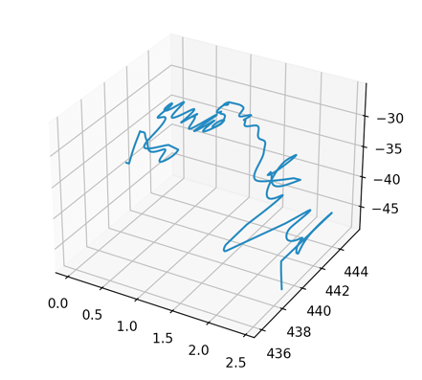
\includegraphics[width=0.8\columnwidth]{pics/one-harm.png}
\caption{3-D plotting of one single harmonic.\label{fig:one-harm}}
\end{figure}

It is necessary to address that if the model is used for analysis purposes, the key points selection will be finished in two steps. To begin with, the positions of the key points are just decided by thresholds on the amplitude and its derivative, but there will be a fine-tuning step after fitting the segment and the intersections of two neighbor segments finalize the detection of the key points in the end. Eventually, the harmonics extracted from a trumpet playing an A4 plotted in Figure \ref{fig:original-harms} can be reconstructed as shown in Figure \ref{fig:synth-harms} with the parameters of frequency and magnitude.

For the phase part whose significance is inasmuch as the prior, we take a traditionally promising method of the Phase Vocoder\cite{flanagan1966phase} for these sine waves with relatively stable frequency. Nevertheless, the vocoder itself is not sufficient for phase generation without specifying the phase for the first time frame for each of the harmonics. Through experiments, we figured out that using either the same constant or a set of randomized take-off phases sounds very unnatural. After taking a closer look at the phase spectrogram of instrument sounds, we discovered that the first frame phases are approximately linear to the frequency. Therefore, it is reasonable to add two more parameters, the slope and the intercept of the linear regression of the first frame phases to anchor the further develop the phase spectrogram.

The last part is the residual. In the HpS model that is mentioned earlier in this section, the morphological feature of the residual part is already depicted by the two subband coefficients. They could be kept since the logic behind them is the same as how the control parameters for the harmonics are chosen. 

Table \ref{tab:parameters} is a summary of the harmonics control parameters. Here in the table, N stands for the number of harmonics that the user puts into. Normally, 20 harmonics already suffice for a good reconstruction of the identity of an instrument, which includes 262 parameters; 40 harmonics, 522 parameters to be exact, are capable of providing a detailed carving of the timbre for low-pitched sounds. In the original spectrogram, if the FFT size is 2048, which is necessary for some low-pitched sounds, the parameter number for a single time frame is already much larger. If we choose the hop size of STFT to be a quarter of the window size, then one second of a sound contains approximately 86 frames, which ends up having 176k complex numbers for one second. Compared to the original signal, the parameter space is significantly more concise and controllable. The operability will be further increased with the graphic interface which will be introduced in the next section.

\begin{figure}[h]
\centering
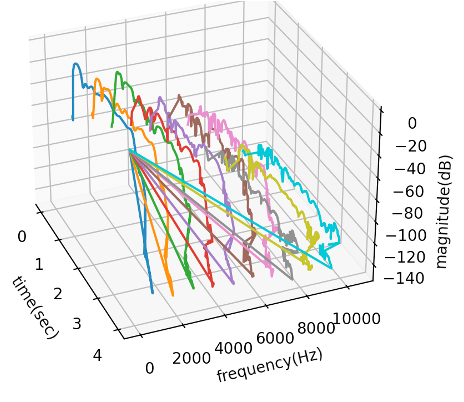
\includegraphics[width=0.8\columnwidth]{pics/flute-org.png}
\caption{First ten harmonics extracted from a trumpet playing a A4. The diagonal lines are caused by the silence at the end of the recording. Both frequency and magnitude are set to zero if no harmonics are detected.\label{fig:original-harms}}
\end{figure}

\begin{figure}[h]
\centering
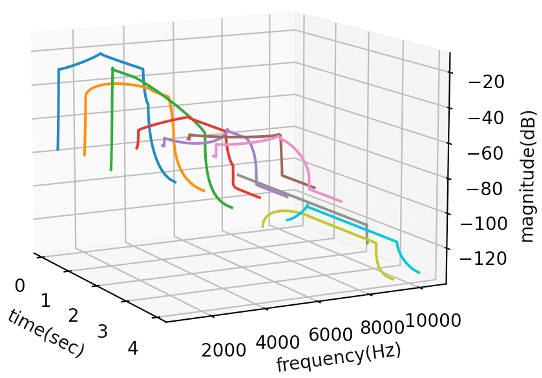
\includegraphics[width=0.7\columnwidth]{pics/flute-synth.png}
\caption{Reconstruction of the ten harmonics given the parameters of frequency and magnitude.\label{fig:synth-harms}}
\end{figure}

\begin{table}[h]
 \begin{center}
 \begin{tabular}{|l|l|}
  \hline
        \textbf{Parameter Name} & \textbf{Parameters amount} \\
        \hline
        Frequency offset mean & N \\
        \hline
        Frequency offset variance & N \\
        \hline
        Magnitude key point time & 4N\\
        \hline
        Magnitude key point magnitude & 4N \\
        \hline
        Magnitude segment shape & 3N \\
        \hline
        Phase of first frames & 2   \\
        \hline
        \textbf{Total} & \textbf{13N+2}\\
        \hline
 \end{tabular}
\end{center}
 \caption{Parameters name and count for N harmonics.}
 \label{tab:parameters}
\end{table}

\subsection{Synthesis Scheme}
With the parameter set, the synthesis scheme is very straightforward. Basically, with the frequency, magnitude, and phase information, the tone can be generated based on an additive synthesis approach. A footnote needs to be added here that for the frequency part, if all of the frequencies are reconstructed independently, then it will excite a noise for the frequent frequency altering. A way to polish that is to concatenate a low-pass filter to smooth out the frequency curve. Users can also modify hyperparameters like the synthesis inverse FFT size and hop size and some other dimensions of a sound like the duration and loudness fairly easily. For the residual part, the envelope shape control parameters can get assigned accordingly depending again on some key points and then do interpolation across time.'
Here are some sound examples of the synthesis result \emph{(the link is omitted for the anonymous requirements)}. 

\subsection{Validity Verification}
To verify the informativity and the validity, we conducted an instrument identification experiment. If the parameters extracted from recordings can distinguish different musical instruments even with very simple classification models, it would be proper to say that this representation really holds the timbre information and has a good spread in the timbre space.

The task we chose here is to classify eight different instruments selected from three orchestra families. We used a random forest with 80 decision trees and had them trained with 1834 audio samples from the audio library of The Philharmonia symphony orchestra\cite{Phiharmonia}. The overall accuracy of the test is 0.81 with a hierarchical classification scheme, which can be considered a good performance for an 8-class classification task. 

We also tested this representation with some synthetic tasks and the results were not disappointing. The tasks include the follows: sound morphing, in which we interpolate between two sounds in the parameter space and yield a gradual timbre shifting from one to the other; pitch shifting, for which we construct the frequencies upon a different fundamental and manage to retain the timbre; and time stretching or shrinking, where we keep all the parameter the same and synthesize simply with a different duration and get a very natural modification. To sum up, this verification tests confirm the validity of the representation and also shows the potential in creative sound design. 

\section{Interface}
This work is expected to be practically user-oriented in the end. To really function as a mediator between technical and non-technical users and the model, we built prototypes for two types of interfaces as a demonstration of both possibilities. The two types of interfaces we implemented are the parameter interface and the graphic interface. Both are developed in Python and have their own strength and use cases.

\subsection{Parameter Interface}
In this interface, all timbre parameters are structured and can be read from and written to json files. An example json file can be found through this link\emph{(the link is omitted for the anonymous requirements)}. The structure comprises two main parts. The first part consists of some hyper-parameters of the synthesis such as the name and id of the file, the Inverse FFT size, the hop size for synthesis, etc. The second part contains all the parameters that are introduced above. In the API, the functions for sound synthesis from json files are implemented, and inversely, there are also functions for feature extraction from a waveform in the API for the users to get more accustomed to the parameter space.

Due to the advantages of the structural data, this form is suitable for some data-driven scenarios, such as analytical tasks, batch processing, and some creative works like sonification projects. For instance, the timbre identification experiment above was conducted through this interface.


\subsection{Graphic Interface}
The other interface form is a graphic GUI that allows visual plotting and interactive manipulation in many different ways. The main window of the interface is shown in the screenshot in Figure \ref{fig:GUI}. It could be tedious to assign every parameter from scratch in a graphic UI, so we approach with a slightly different strategy we take here is to first import either a sound or a json file as a starting point. The plottings on the left show the spectrogram and harmonics in 3D for both the current modification of the sound and the original imported sound as a comparison. All the parameters can be modified with the input boxes on the right, and the modifications can reflect on the graphs per process. A more illustrative way of reshaping the harmonics is by dragging the key points directly on a canvas. If selecting the corresponding number of the harmonic and clicking on the \emph{drag key points} button, a separate window like Figure \ref{fig:GUI-drag} will pop out for interactive modification. The bottom right section in the main window embeds the sound morphing tool which is mentioned in the previous session. An introduction video can be found through this link \emph{(the link is omitted for the anonymous requirements)}.


\begin{figure}[h]
\centering
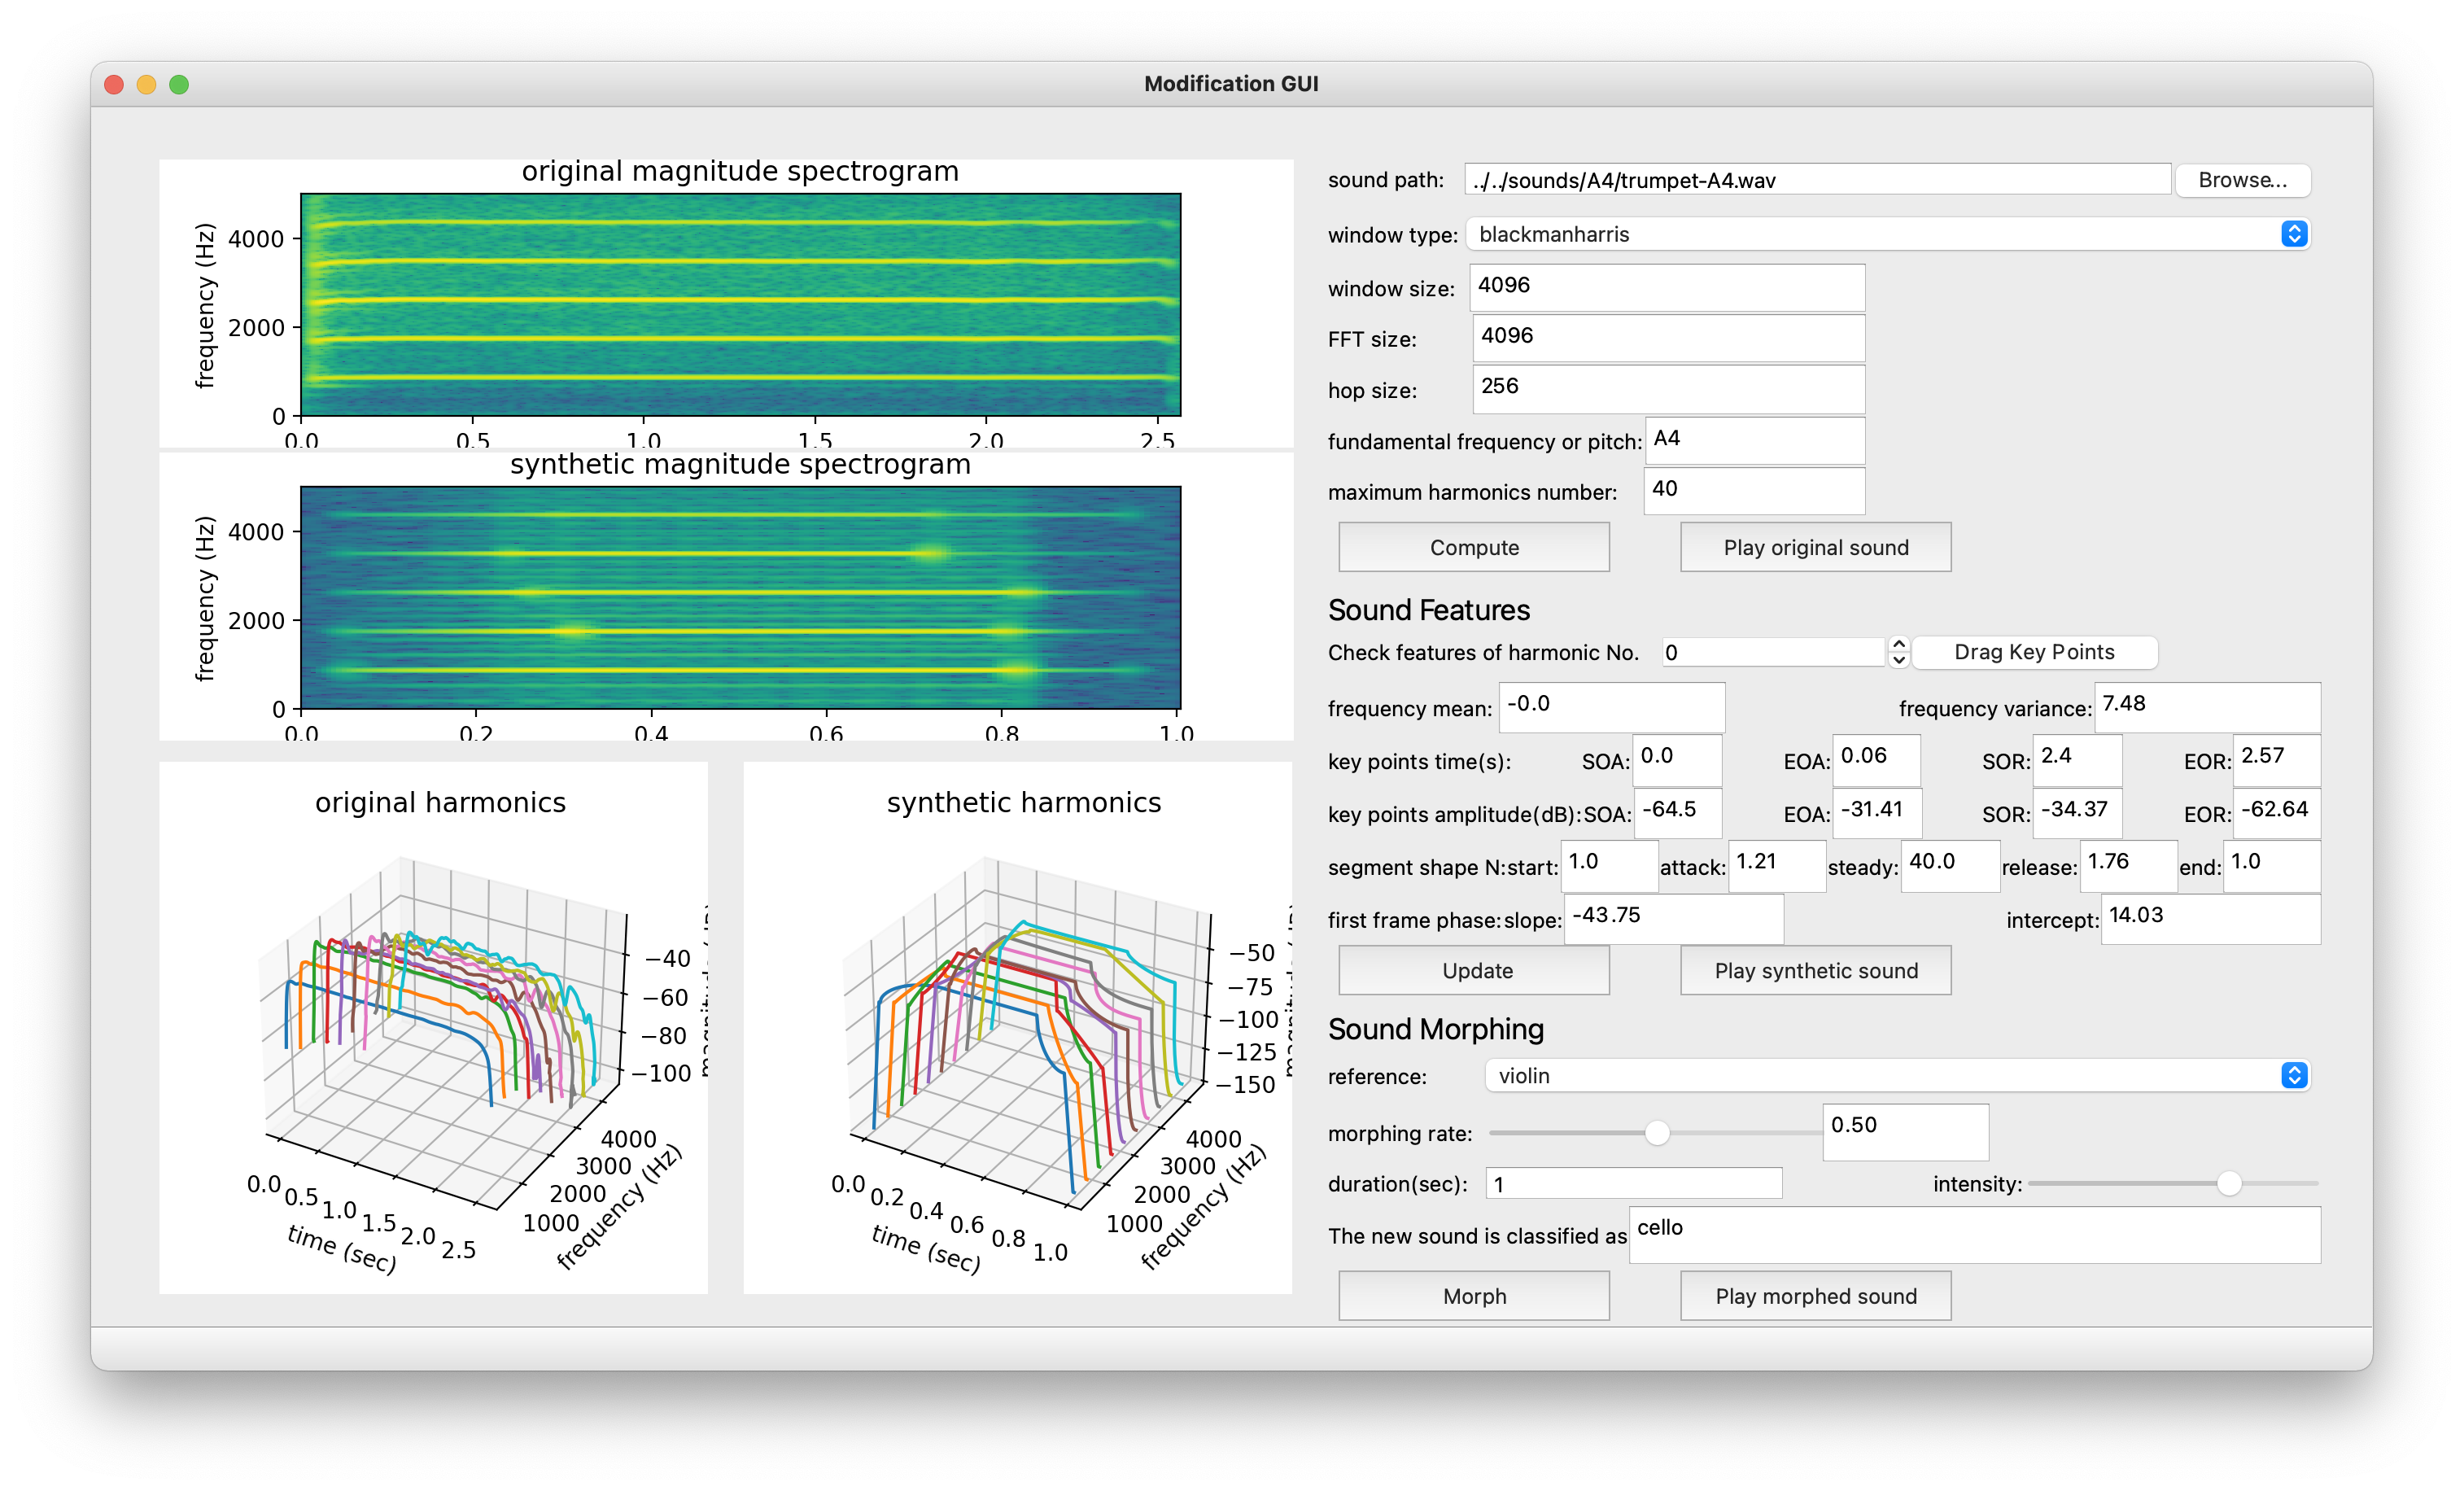
\includegraphics[width=0.9\columnwidth]{pics/GUI.png}
\caption{The main UI of the graphic interface.\label{fig:GUI}}
\end{figure}

\begin{figure}[h]
\centering
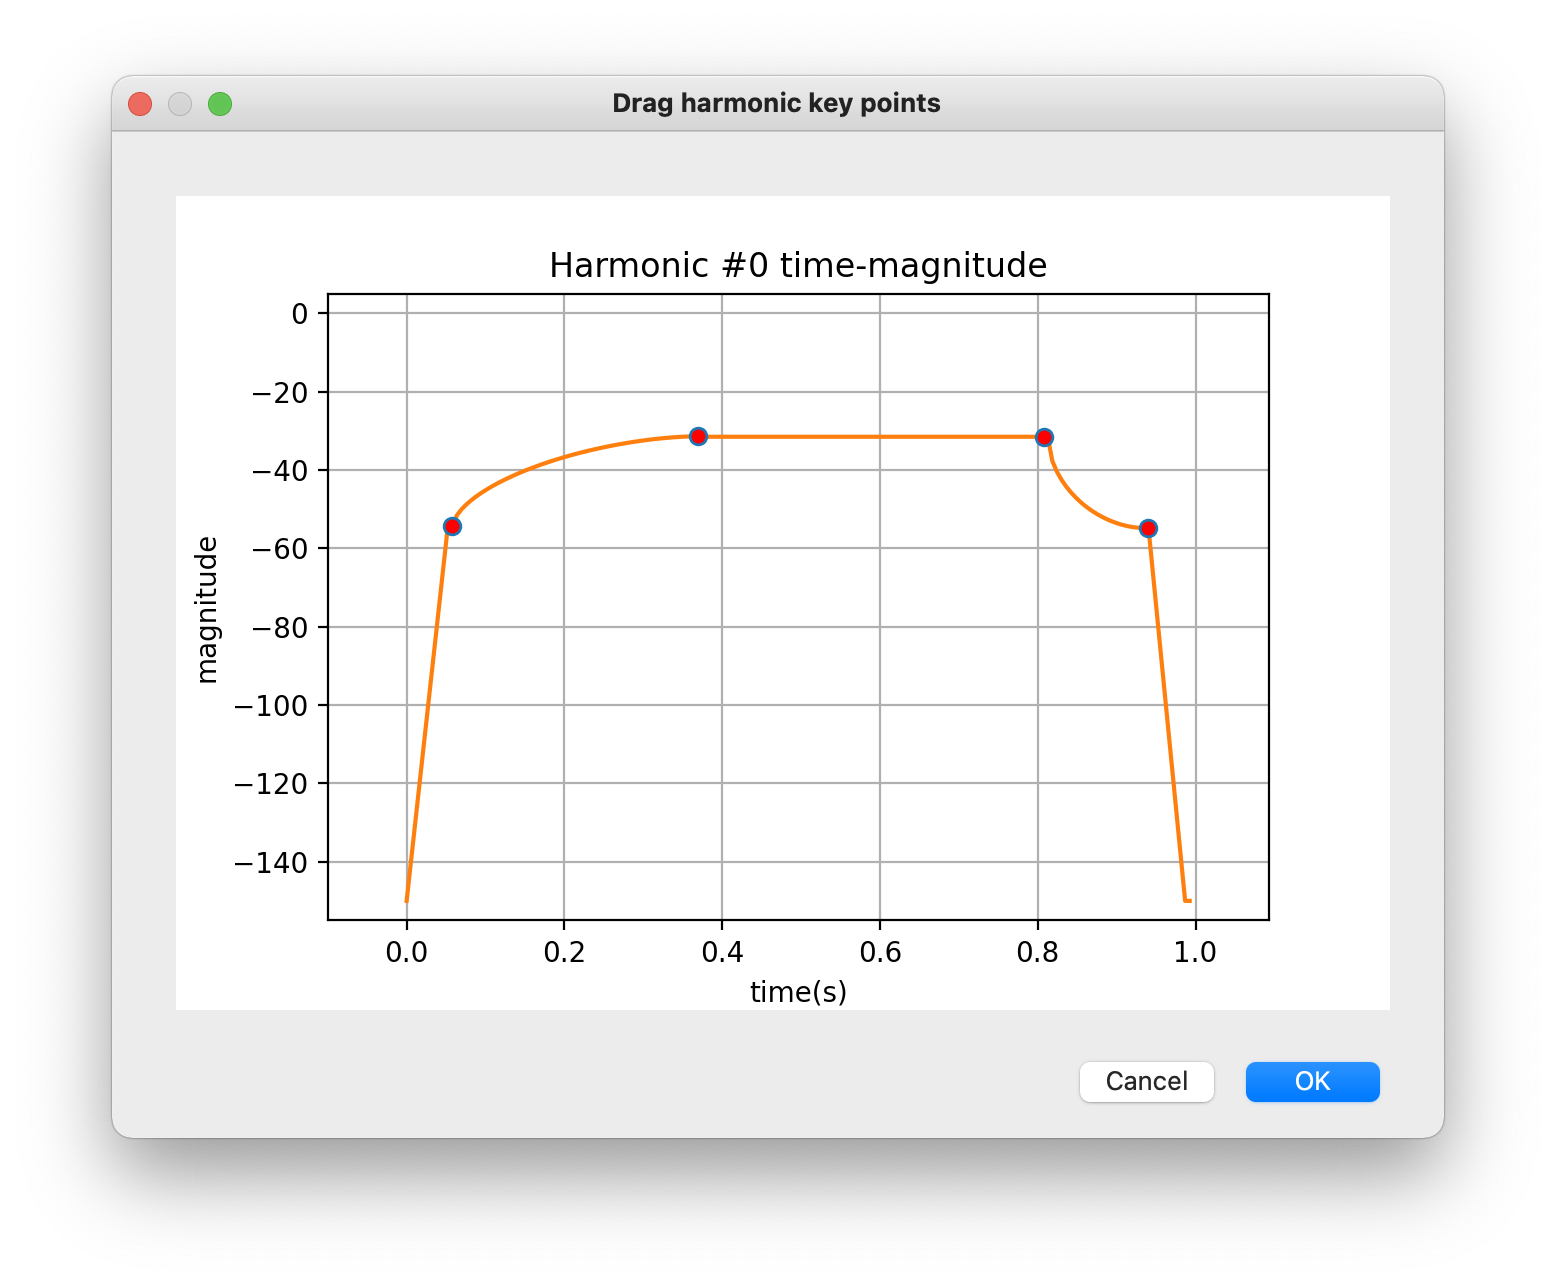
\includegraphics[width=0.9\columnwidth]{pics/GUI-drag.png}
\caption{The child window that pops out when the \emph{'drag key point'} button is clicked In this interactive window, users can drag the key points in the plotting and make a real-time modification of the curve.\label{fig:GUI-drag}}
\end{figure}


\section{Discussion}
% \subsection{Future of Spectral Modeling and Synthesis}
This work inherits a lot of previous works on spectral modeling of musical timbre as a summary and an extension of some of the most fundamental and significant models. It distills semantically understandable and controllable features from the chaotic spectrogram and empowers the parameters with synthetic functions. Actually, the problem that the work points out is equally worth discussing as the work per se. It is undeniable that the spectrogram comprises nearly all of the information in a waveform, however the question being asked here is how to set people free from the constraints brought by existing sounds and sound design approach, and thoroughly utilize the spectrogram as a primary tool till a degree that people can think of sound and design sound mainly from its spectral character. That is to say, we need comprehensive semantic control parameters like the effort made in this work, but more importantly, we need a better understanding of timbre to design the parameters. 

After decades of research, timbre still remains an open question. This question can hardly be answered by deep learning approaches due to their own defects in interoperability, and on the other hand, the conventional descriptors which are still commonly used today in timbre-related research also find their limit as discussed in the beginning. After all, the understanding and the tool are improving alternatingly, so we conduct analysis on the synthesis results and refine synthesis based on the analysis. The control parameters proposed in this work serve for the synthesis half but point towards analysis aims as well. It echoes all acoustic-related tasks that hope to take timbre into account and functions as a bridge connecting the visuals with the sound for all types of data and projects too. With all of the potential, spectral modeling should be continued and put at the center of sound synthesis research again.

% \subsection{Echoing other acoustic tasks}


% \subsection{As a bridge connecting vision and auditory}


\begin{acknowledgments}
% While working on this project and composing this paper, it was impossible not to think about and pay homage to the pioneering researchers and musicians who came before us. We should feel privileged to be living in a time when we can understand sound at such a composed level thanks to their visions and insights. I would like to dedicate this paper to Julius Smith, whose contributions to spectral modeling and generous help and instruction were invaluable to me when I was just starting out as a random engineering student. Finally, I would like to express my heartfelt thanks to my friends Zehao Wang and Yifan Guo, without whose encouragement and company this project would never have been possible.
\end{acknowledgments} 

%%%%%%%%%%%%%%%%%%%%%%%%%%%%%%%%%%%%%%%%%%%%%%%%%%%%%%%%%%%%%%%%%%%%%%%%%%%%%
%bibliography here
\bibliography{icmc2023template}

\end{document}
